\section{Evaluation}

% Evaluation Setup
% \section{Implementation}

\subsection{Implementation and Evaluation Setup}
\begin{figure}
    \centering
    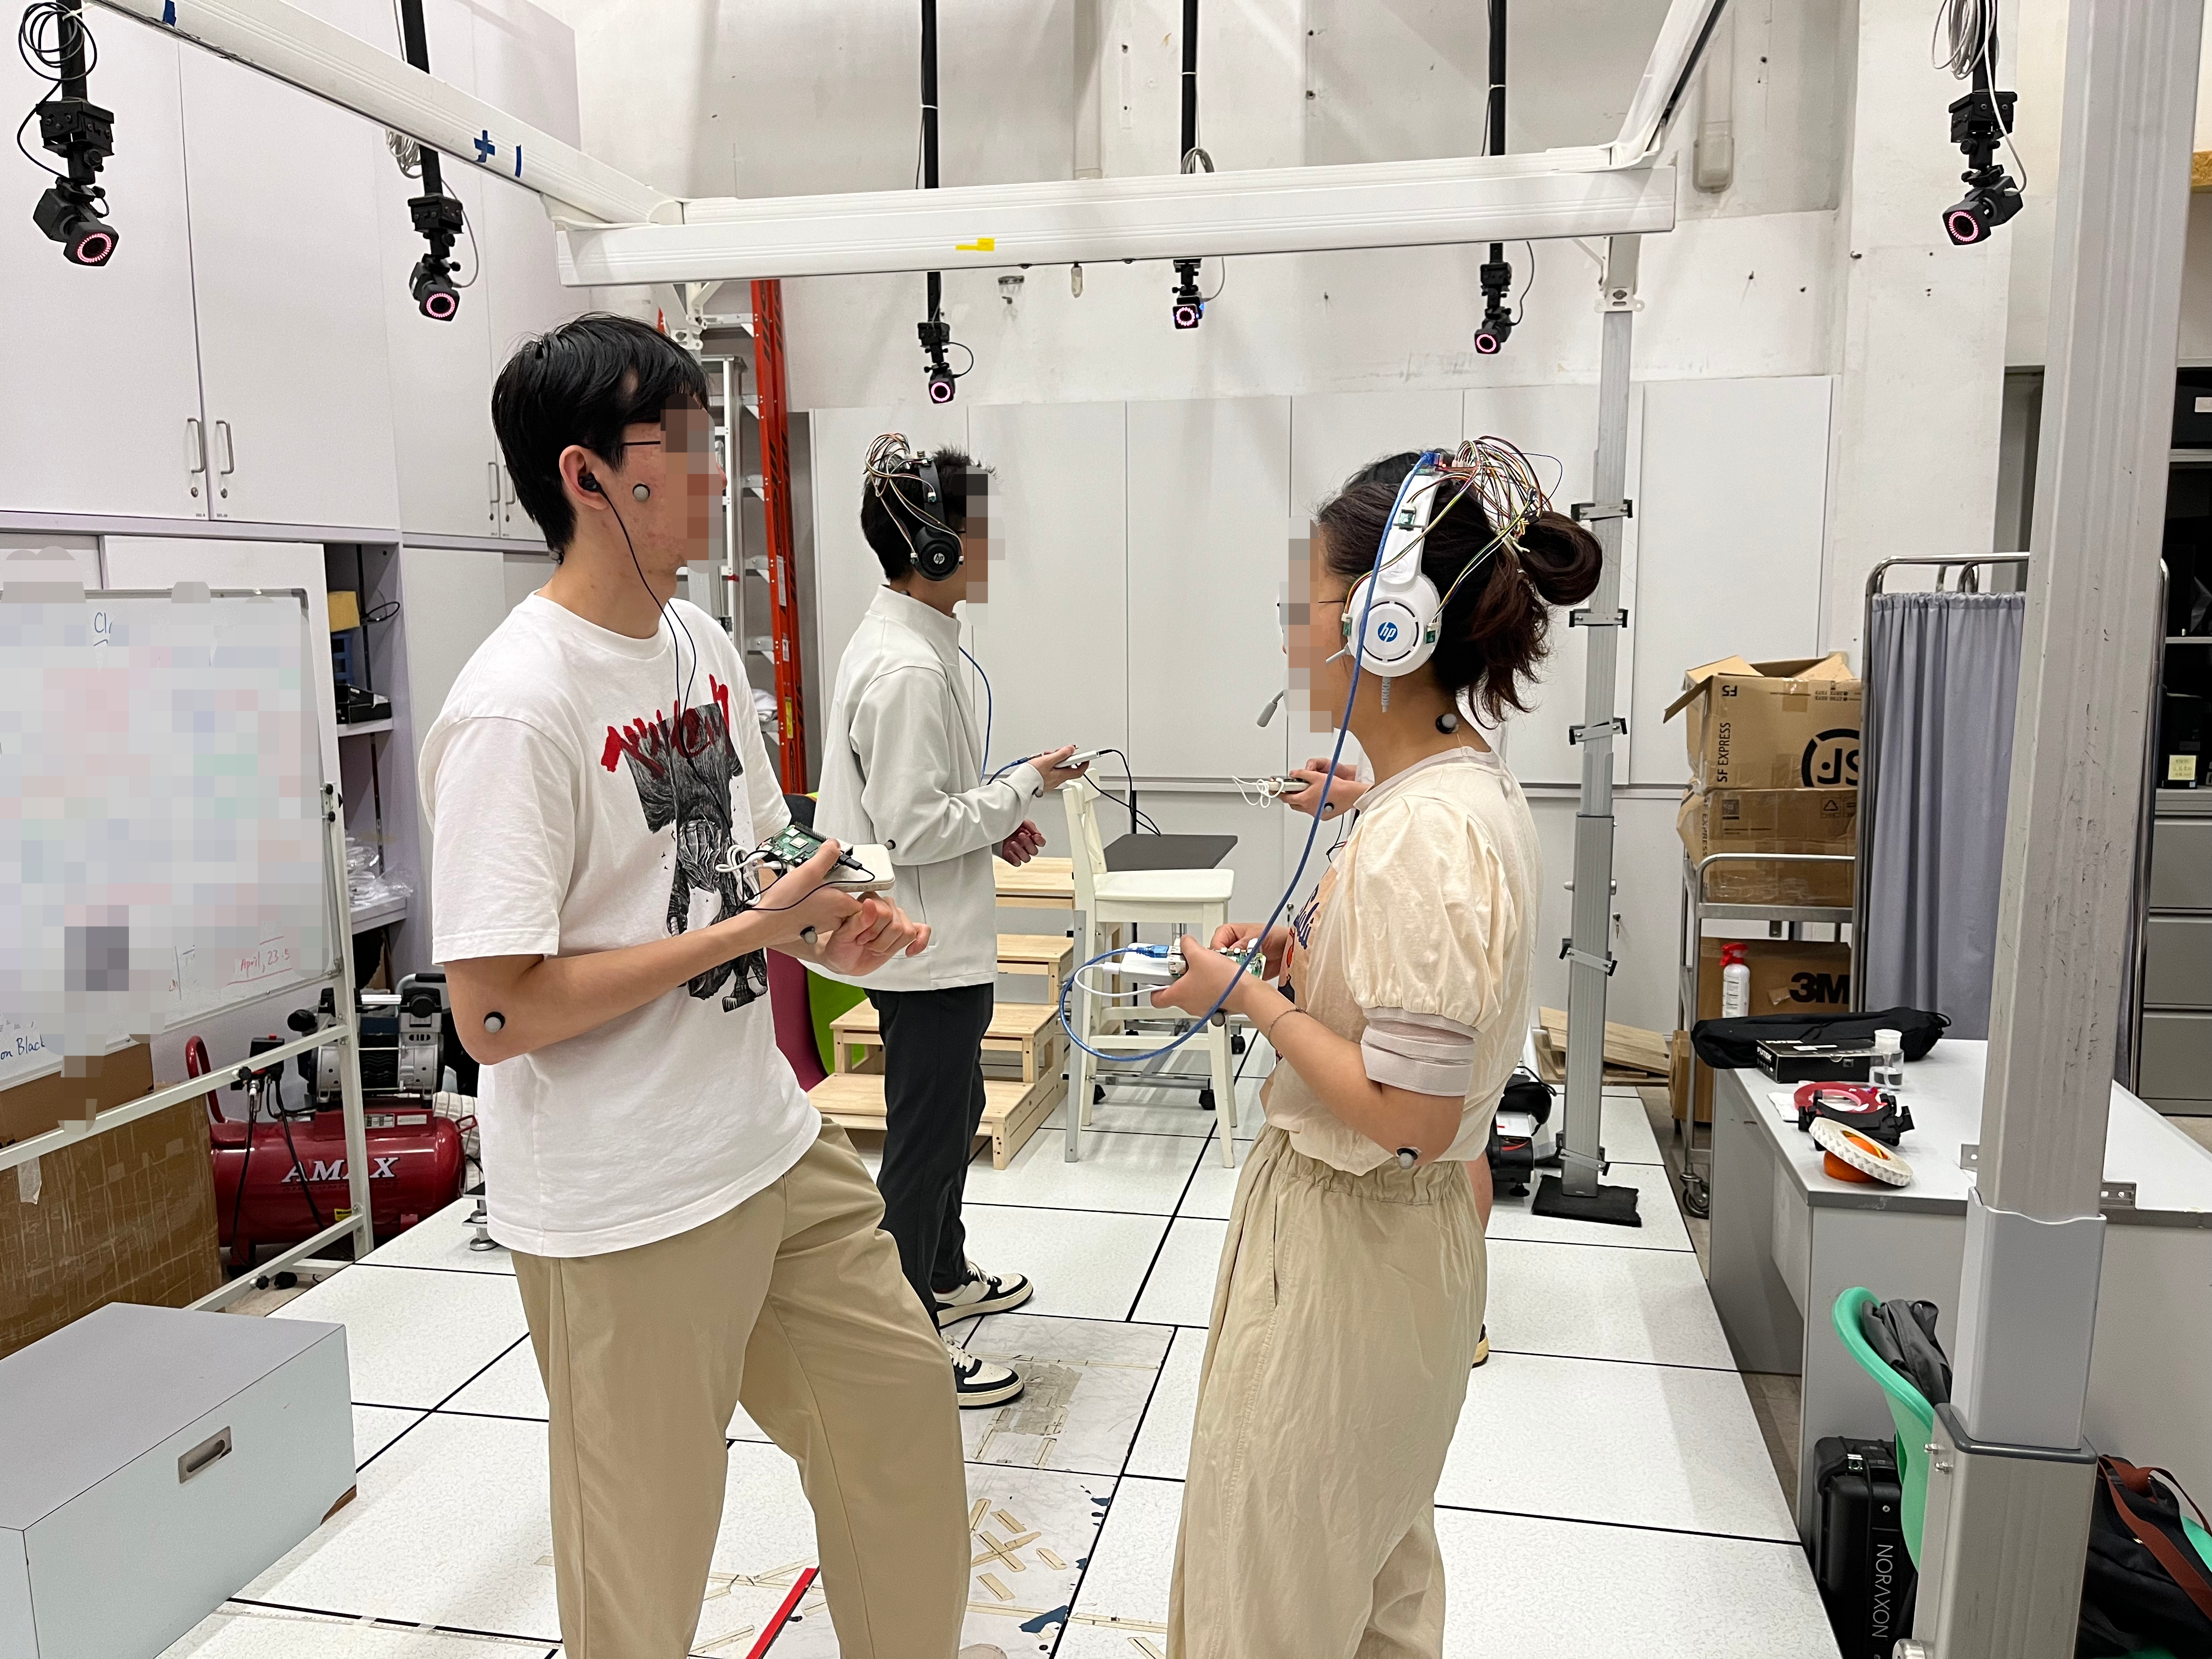
\includegraphics[width=0.5 \linewidth]{chapters/cohear/figs/experiment.png}
    \caption{Experiment setup of the motion capture room.}
    \label{fig:mocap}
    \vspace{-1em}
\end{figure}


\paragraph{Testbed Setup}
\label{sec:cohear_hardware}
We implement CoHear in various form factors, including binaural earphones and headphones with up to an 8-channel microphone array (placement is illustrated in Fig. \ref{fig:mic_loc}). The two earphones are shown in Fig. \ref{fig:hardware}. We use a Raspberry Pi 5 to collect audio and attach one IMU (BMI-160) to the headphones to track head motion, transmitted via I2C. For experimental validation, we connect each device via SSH under the same WiFi network, streaming all data to a desktop for analysis. The system output is designed to be played back through the headphone speakers, maintaining compatibility with existing ANC functionality. 

While our hardware supports sampling rates up to 48 kHz for maximum capture capability, the system is designed to operate at lower rates suitable for real-world deployment.
For practical speech applications, CoHear can operate at 8 kHz with audio compression to minimize bandwidth requirements, which is also evaluated in the later section.
Moreover, CoHear supports time-invariant speaker embeddings that require only one-time transmission, significantly reducing data size to 8192 bits in total, which is practical on even constrained networks. We also discuss the networking issue in Sec. \ref{sec:cohear_discuss}.


\begin{figure}[t]
    \centering
    \begin{minipage}{0.48\linewidth}
    \centering
    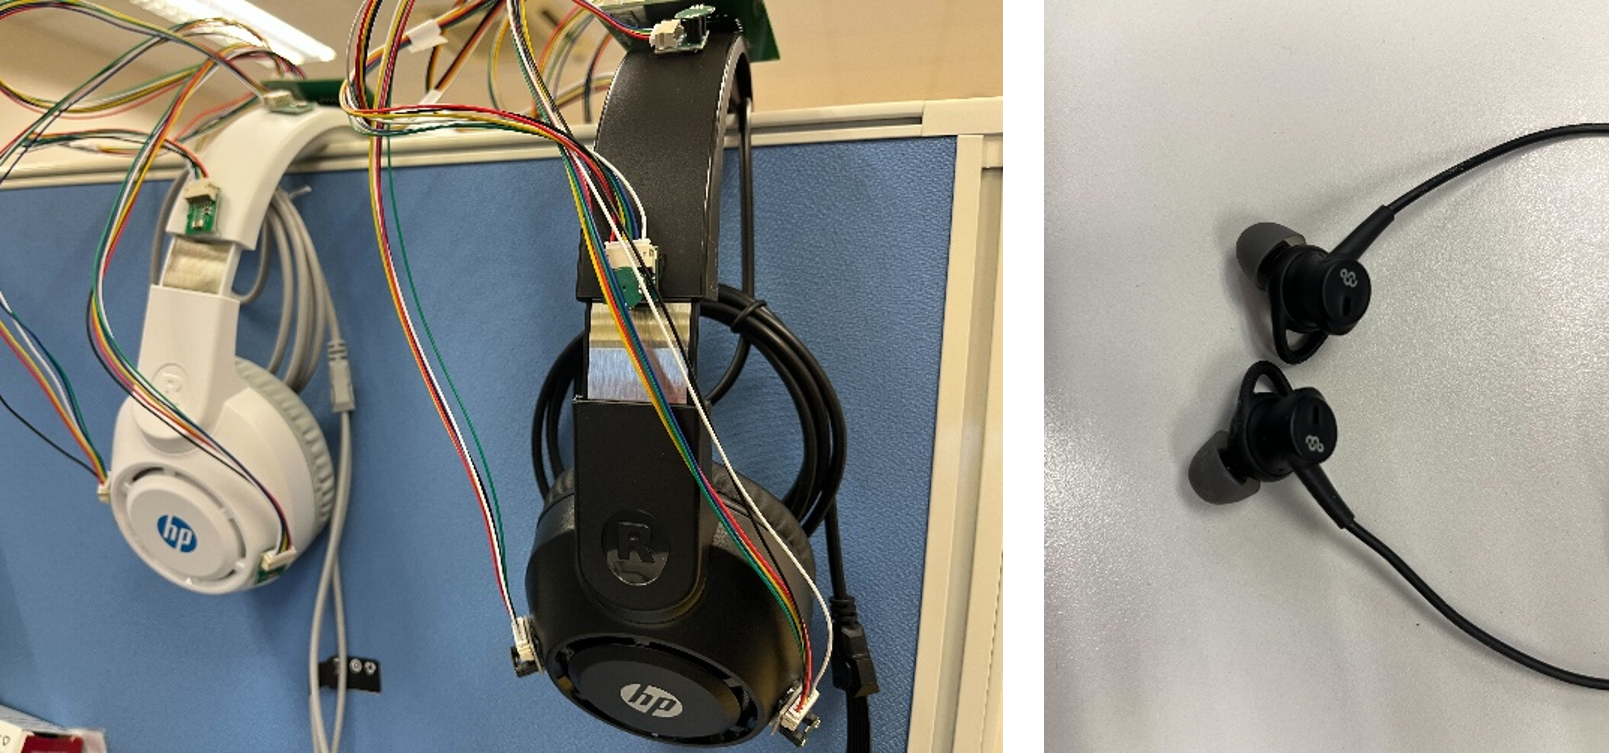
\includegraphics[width=0.8\linewidth]{chapters/cohear/figs/device.png}
    \caption{Hardware used in the experiment.}
    \label{fig:hardware}
    \end{minipage}
    \hfill
     \begin{minipage}{0.48\linewidth}
        \centering
        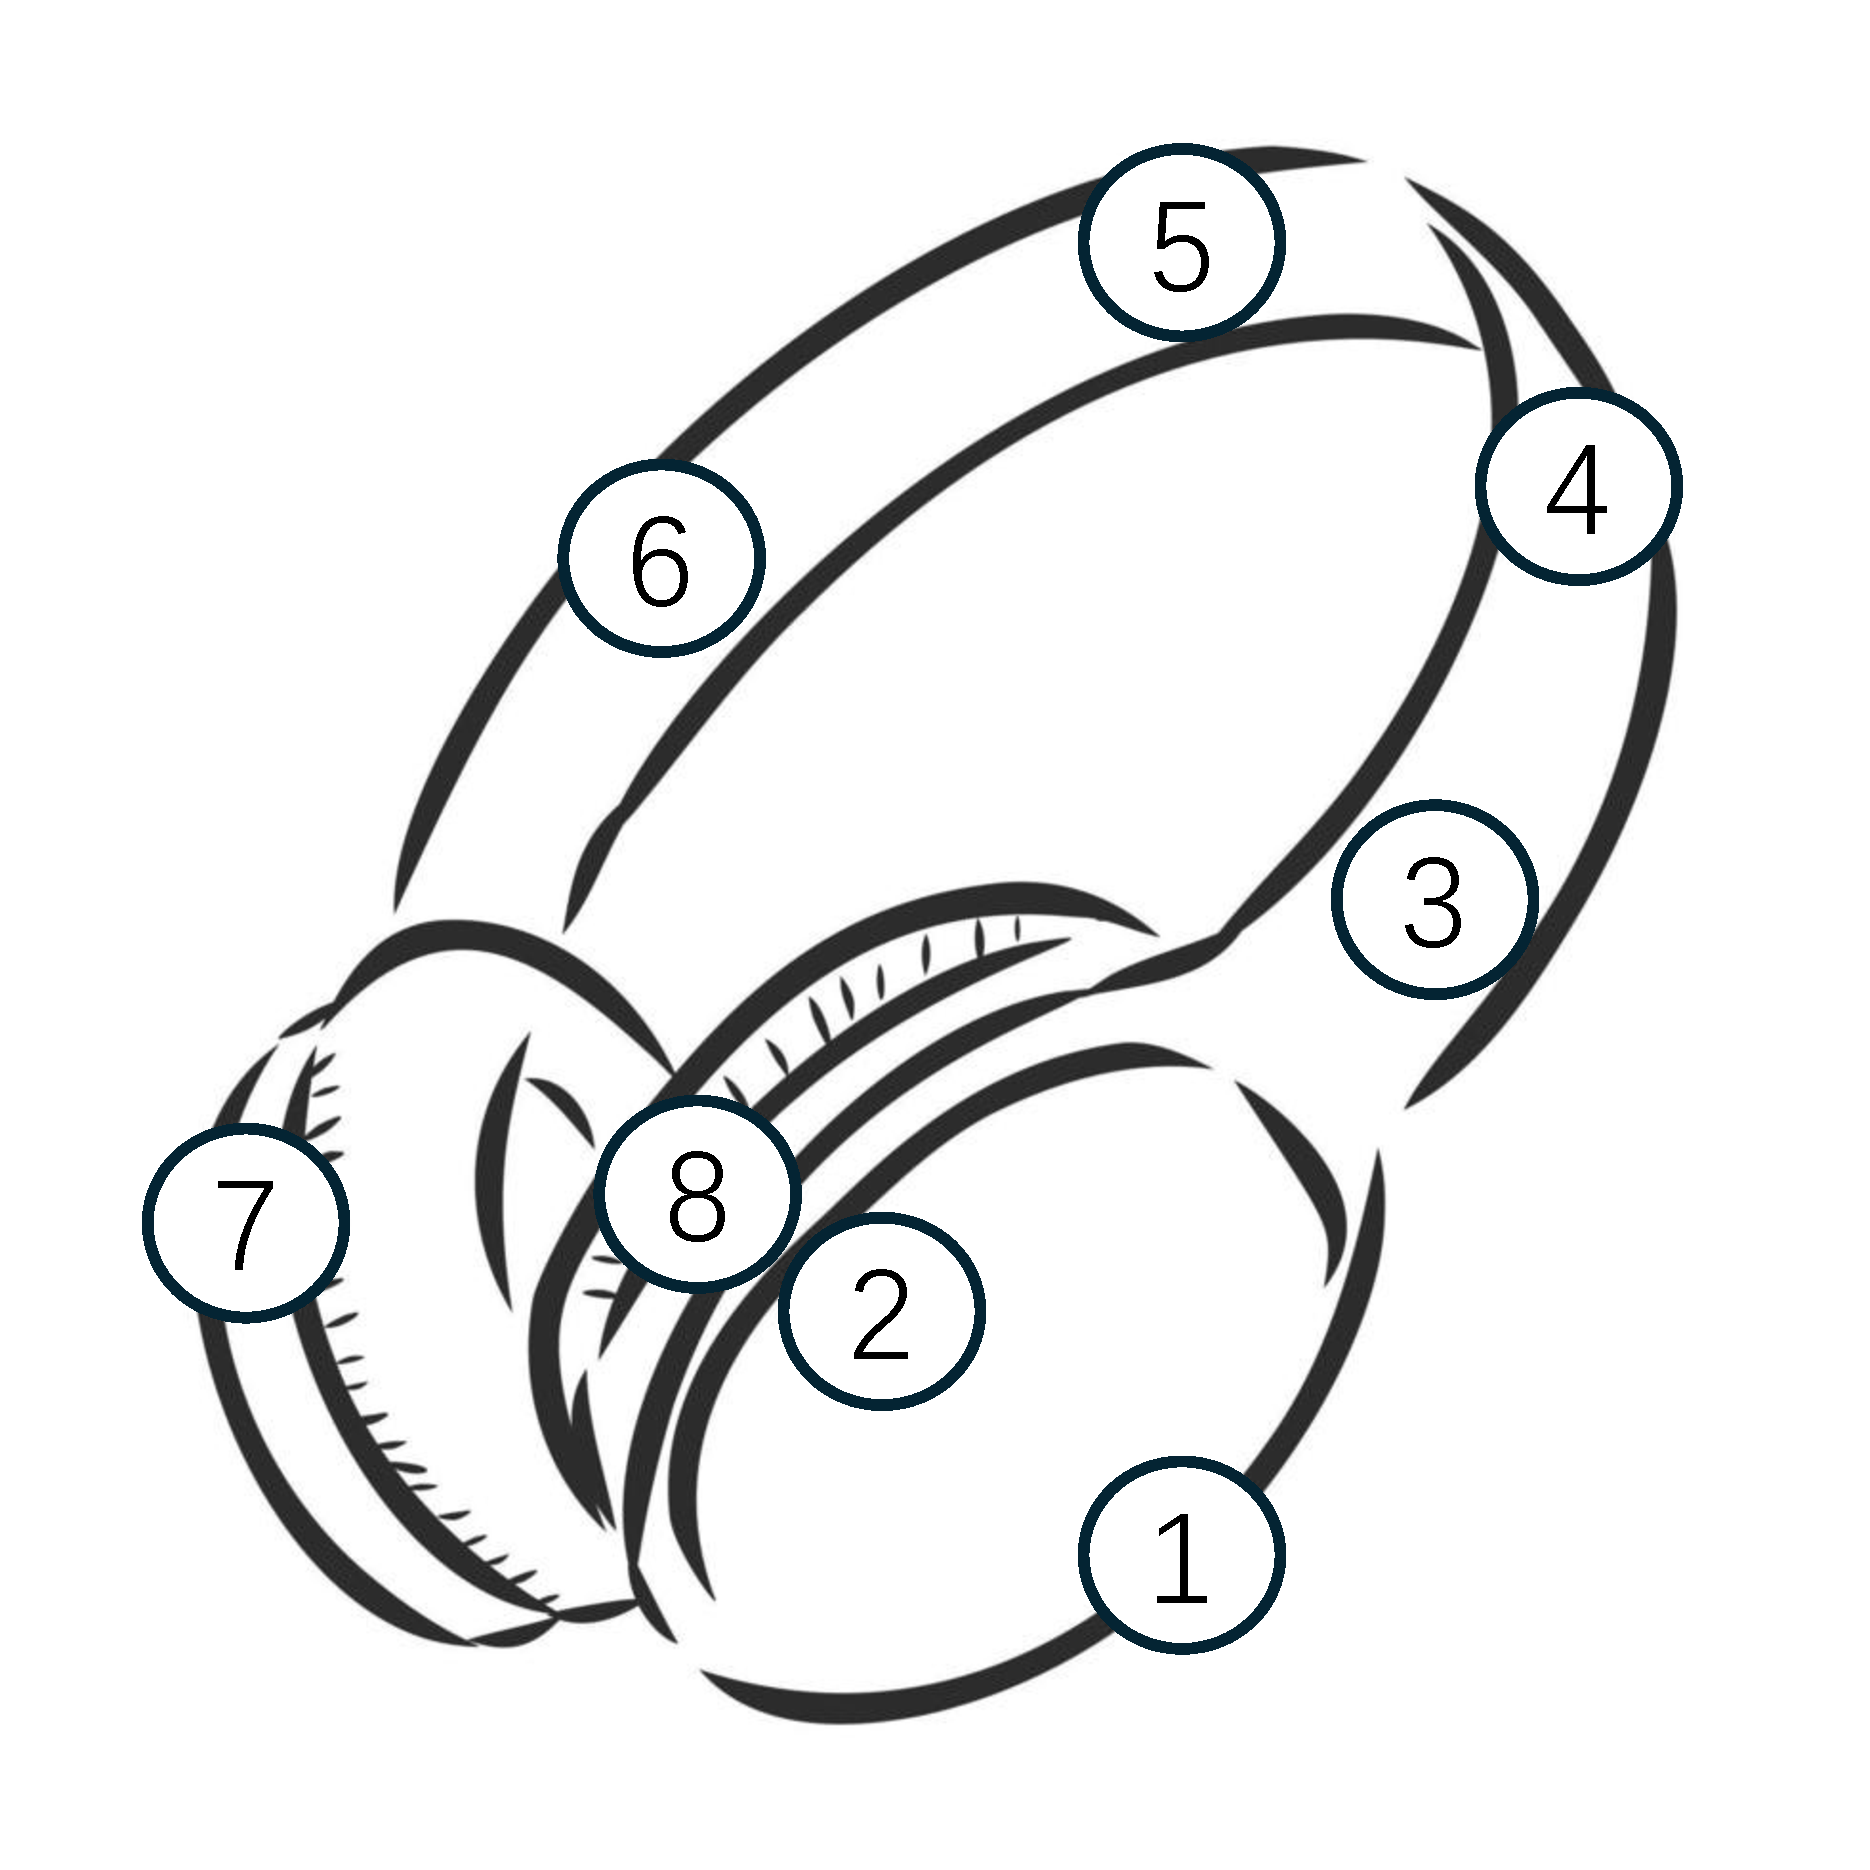
\includegraphics[width=0.4\linewidth]{chapters/cohear/figs/mic_loc.pdf}
    \caption{Microphones location on the headphone.}
    \label{fig:mic_loc}
    \end{minipage}%
    \vspace{-1em}
\end{figure}


\paragraph{Dataset Collection}
We use three data sources to support the design and evaluation of CoHear: a real-world dataset collected in a motion capture room, simulated datasets for large-scale testing and training, and public datasets for comparison.

\vspace{1ex}
\noindent\textit{Real-world Collection:}
We collected 30 minutes of multi-person conversation data in a $10 \times 5$ m motion capture room equipped with a 12-camera VICON system (Fig.~\ref{fig:mocap}). Markers were placed on participants’ heads and upper bodies to track conversational poses. Six volunteers wore our prototype headphones (Section~\ref{sec:cohear_hardware}) and engaged in natural turn-taking conversations. Due to space limitations, each session involved 2–4 participants in different grouping scenarios:
1) two participants in one group,
2) three participants with one excluded, and
3) four participants split into two groups.

\vspace{1ex}
\noindent\textit{Simulation:}
To scale beyond the limits of physical collection, we simulate two datasets: 1) Geometric Calibration: Using Pyroomacoustics~\cite{scheibler2018pyroomacoustics}, we simulate dynamic conversations in larger rooms (up to 20 m wide) with varied reverberation (RT60 from 0.25 to 0.75).
And 2) Conversation Extraction: We augment the real dataset with noisy-clean pairs and degraded relays (e.g., SNR, compression, bit crush, packet loss) to train and evaluate the enhancement model. The SNR of the noisy speech is set to between -10 dB and 10 dB.

\vspace{1ex}
\noindent\textit{Public Datasets:}
We also compare CoHear with existing datasets in Table~\ref{tab:comparison_dataset}. While prior work such as STARSS23~\cite{shimada2024starss23} and 6DoF-SELD~\cite{yasuda20246dof} focuses on sound event localization, and AMI~\cite{kraaij2005ami} and EasyCom~\cite{donley2021easycom} cover conversations, none support collaborative multi-device conversation modeling with 6DoF tracking as CoHear does.

\begin{table}[t]
\caption{Comparison with existing datasets.}
\centering
\begin{tabular}{|c|c|c|c|}
\hline
\textbf{Name} & \textbf{6DoF} & \textbf{Multi-device} & \textbf{Target} \\
\hline
STARSS23~\cite{shimada2024starss23} & No & No & Sound events \\
6DoF-SELD~\cite{yasuda20246dof} & Yes & No & Sound events \\
AMI~\cite{kraaij2005ami} & No & No & Conversation \\
EasyCom~\cite{donley2021easycom} & Yes & No & Conversation \\
\textbf{CoHear} & \textbf{Yes} & \textbf{Yes} & \textbf{Conversation} \\
\hline
\end{tabular}
\label{tab:comparison_dataset}
\end{table}



\paragraph{Evaluation Metrics}
The primary objectives of CoHear are to identify user locations and extract relevant conversations, assessed through distinct metrics.

For geometric calibration, we use two standard metrics: average direction error (in degrees) and location error (in meters). We also incorporate network setup accuracy, which indicates whether the participant can find the correct partner. Specifically, we define \(S_{i,j}\) equals to true if \(|R_{i,j} - O_i| < \frac{\pi}{4}\), where \(R_{i,j}\) is the relative direction from user \(j\) to user \(i\) and \(O_i\) is the orientation of user \(i\). 

As for the conversation enhancement, we will utilize the scale-invariant signal-to-noise ratio (Si-SNR) as a conversation-related metric, noting that the input SNR significantly influences results. Since the average default input SNR is set to 0 dB, allowing the output SNR to reflect improvements over the input.

\paragraph{Baselines Approaches}
Similar to the metrics, we also incorporate different baselines for the geometric calibration and conversation extraction, respectively.
For the former one, we consider \cite{gburrek2021geometry} as the baseline, which is designed for static WASN only. Besides, infrastructure-based acoustic localization \cite{gburrek2021geometry} and acoustic-SLAM \cite{evers2018acoustic} are related to CoHear. Note that when we apply \cite{gburrek2021geometry} as infrastructure-based acoustic localization, we have static nodes but mobile sources (i.e., users); our target becomes estimating the sound sources rather than nodes. We will use the following abbreviations in this paper: DSM refers to baseline \cite{gburrek2021geometry}, iDSM refers to infrastructure-based acoustic localization \cite{gburrek2021geometry}, and aSLAM for acoustic-SLAM \cite{evers2018acoustic}.


As for the conversation extraction, we consider LookOncetoHear \cite{veluri2024look}, target conversation extraction \cite{chen2024target}, and CoS \cite{jenrungrot2020cone} as our baselines. We also replace the relay audio with time-dependent speaker embedding as a baseline.
For LookOncetoHear \cite{veluri2024look}, we assume the enrollment happened in every sentence and takes effect in the next sentence. For the second baseline, we consider self-voice to be the condition. As for the CoS \cite{jenrungrot2020cone}, we assume the interferences span randomly in the nearby space while the target speaker is always in front of the user.
We will use the following abbreviations in this paper: LOTH stands for LookOnceToHear \cite{veluri2024look}, TC refers to \cite{chen2024target}, CoS refers to \cite{jenrungrot2020cone}



\begin{figure}
    \centering
    \begin{subfigure}{0.48\linewidth}
        \centering
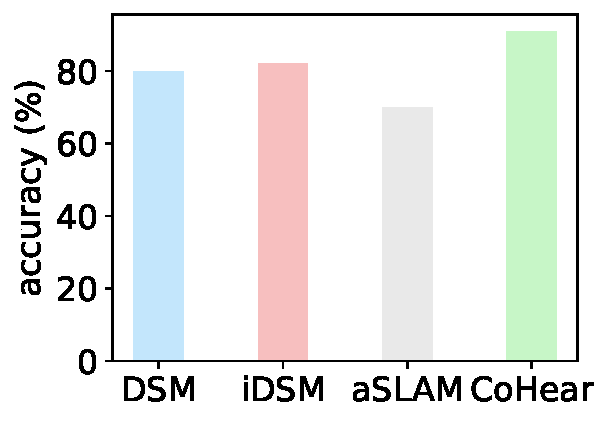
\includegraphics[width=0.75\linewidth]{chapters/cohear/evaluation/calibration_output_accuracy.pdf}
        \caption{Network topology accuracy.}
        \label{fig:topology accuracy}
    \end{subfigure}%
    \begin{subfigure}{0.48\linewidth}
        \centering
        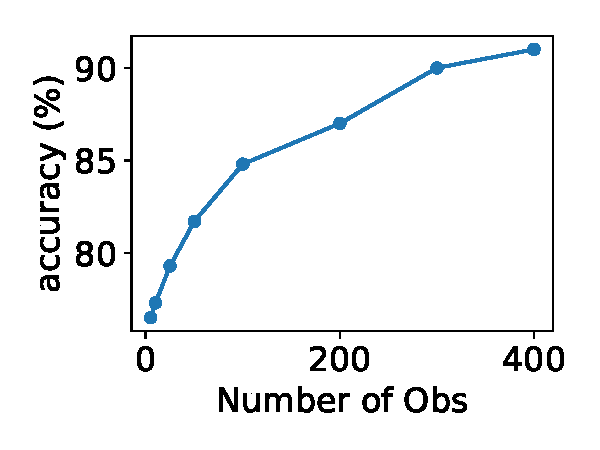
\includegraphics[width=0.75\linewidth]{chapters/cohear/evaluation/num_obs_accuracy.pdf}
        \caption{Network topology accuracy with increasing observations.}
        \label{fig:topology accuracy_obs}
    \end{subfigure}%
     \vspace{-1em}
  \caption{Conversation setup performance.}
   \vspace{-1em}
\label{fig:topology}
\end{figure}

\begin{figure}
    \centering
    \begin{subfigure}{0.48\linewidth}
        \centering
        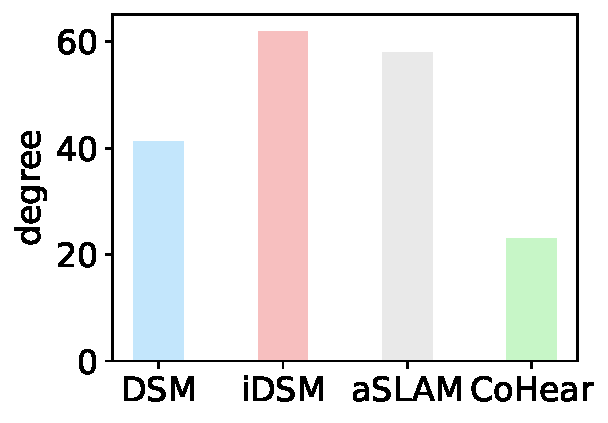
\includegraphics[width=0.75\linewidth]{chapters/cohear/evaluation/calibration_output_orientation.pdf}
        \caption{Orientation errors.}
        \label{fig:calibration_output_ori}
    \end{subfigure}%
    \begin{subfigure}{0.48\linewidth}
        \centering
        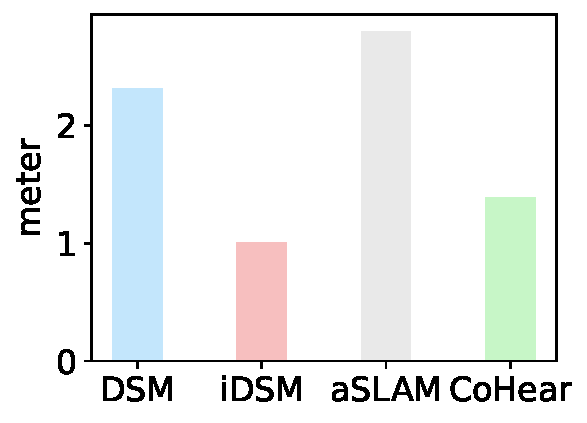
\includegraphics[width=0.75\linewidth]{chapters/cohear/evaluation/calibration_output_position.pdf}
        \caption{Position errors.}
        \label{fig:calibration_output_pos}
    \end{subfigure}%
      \vspace{-1em}
  \caption{Performance on geometric calibration.}
\label{fig:calibration_output}
\vspace{-1em}
\end{figure}


\subsection{System Performance}

\paragraph{Conversation detection}
We compare CoHear with three previously introduced baselines in terms of connection setup, as shown in Fig. \ref{fig:topology accuracy}. Overall, CoHear outperforms all the baselines by up to 20\%, achieving over 90\% accuracy in detecting connections. This demonstrates its effectiveness in successfully establishing the network.
In addition, we present the accuracy across different observation counts in Fig. \ref{fig:topology accuracy_obs}. Here, we can see that the accuracy starts at 76\% with just five observations and eventually increases to over 90\% as more observations are included.

\paragraph{Geometric calibration}
We compare CoHear with three baselines we introduced before in Fig. \ref{fig:calibration_output}. Overall, CoHear outperforms all the baselines except for position errors compared to iDSM. However, iDSM is an infrastructure-based solution with much higher deployment overhead. In summary, CoHear reduce the orientation errors up to 43\% and up to 28\% for position errors.

\begin{figure}
    \centering
    \begin{subfigure}{0.48\linewidth}
        \centering
        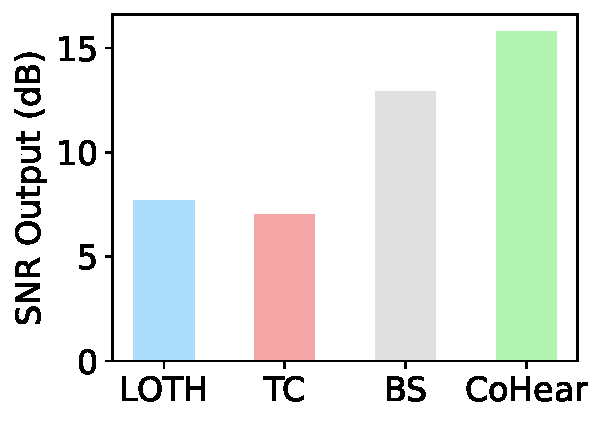
\includegraphics[width=0.75\linewidth]{chapters/cohear/evaluation/snr_output.pdf}
        \caption{Compared to baselines.}
        \label{fig:compare_speech}
    \end{subfigure}%
    \begin{subfigure}{0.48\linewidth}
        \centering
        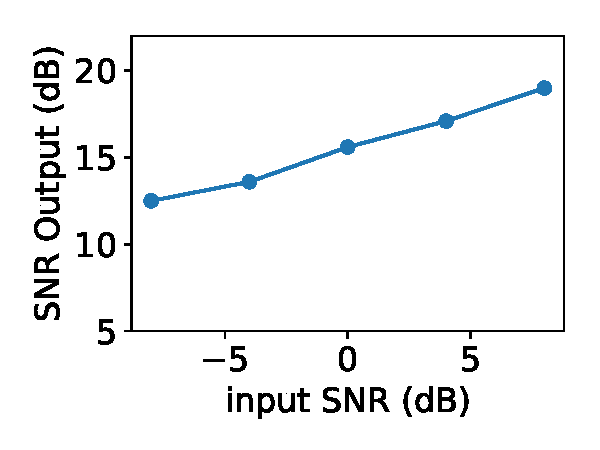
\includegraphics[width=0.75\linewidth]{chapters/cohear/evaluation/input_snr.pdf}
        \caption{Performance with different input SNR.}
        \label{fig:input_snr}
    \end{subfigure}%
     \vspace{-1em}
    \caption{Performance on conversation extraction, }
    \label{fig:compare}
        \vspace{-1em}
\end{figure}

\paragraph{Conversation extraction}
We compare CoHear against the three baselines illustrated before, as shown in Fig. \ref{fig:compare}. We observe that CoHear outperforms them with large margin, especially for LOTH (8dB improvement) and TC (8.8dB improvement). As for the CoS, CoHear obtains better performance without knowing the location of the speaker, enabling more flexible applications.
The performance of the speech filter also correlates with the input SNR. Apparently, the higher the SNR of the input, the higher the SNR of the output. In the previous evaluation, we already used the difference between input and output to avoid bias. However, it is still interesting to observe the performance under different levels of input SNR in Fig. \ref{fig:input_snr}.

\begin{figure}
    \centering
    \begin{subfigure}{0.48\linewidth}
        \centering
        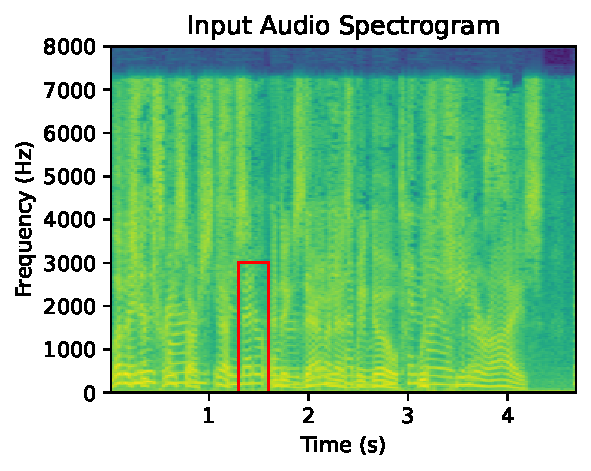
\includegraphics[width=1\linewidth]{chapters/cohear/evaluation/spec_input.pdf}
        \caption{Spectrogram of the input noisy speech.}
        \vspace{-1em}
        \label{fig:visual_input}
    \end{subfigure}%
    \begin{subfigure}{0.48\linewidth}
        \centering
        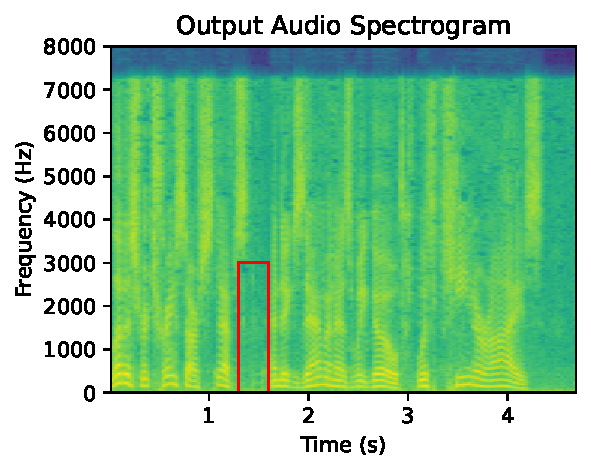
\includegraphics[width=1\linewidth]{chapters/cohear/evaluation/spec_output.pdf}
        \caption{Spectrogram of the output of CoHear.}
        \vspace{-1em}
        \label{fig:visual_output}
    \end{subfigure}%
     
    \caption{Spectrograms of speech before and after the processing, the red box highlights the interference which is desired to be removed. The speech content is ``Let us retrace our steps...''.}
    \label{fig:visual}
    \vspace{-1em}
\end{figure}

\paragraph{Visual analysis}
In addition to the results we presented using conventional metrics, we also show the input and output of CoHear in Fig. \ref{fig:visual}. In the input spectrogram depicted in Fig. \ref{fig:visual_input}, we notice significant overlap of speech sounds, which occur at nearly the same frequency band. However, with CoHear, the interfering speech is effectively removed, as illustrated in Fig. \ref{fig:visual_output}. To enhance clarity, we have highlighted the noise in both figures with a red box, and we can observe that it disappears in the output shown in the right figure.


\paragraph{Ablation Study}
\begin{table}
    \centering
    \caption{Ablation Study for Geometric Calibration}
     \vspace{-1em}
    \begin{tabular}{|l|c|c|}
        \hline
        \textbf{Ablation Component} & \textbf{Position (m)} & \textbf{Orientation (°)} \\
        \hline
        Distance Only & 3.61 & 86.65 \\
        \hline
        Naive Distance & 2.2 & 41. \\
        \hline
        Weight Optimization & 1.69 & 37 \\
        \hline
        CoHear & 1.39 & 23.1 \\
        \hline
    \end{tabular}
    \label{tab:ablation_calibration}
        \vspace{-1em}
\end{table}
We conducted an ablation study on geometric calibration by assessing three key components: 1) direction of arrival, 2) collaborative distance estimation, and 3) weight optimization, as shown in Table \ref{tab:ablation_calibration}. Our findings indicate that all three components significantly contribute to the final results. When we used distance estimation as the only observation for calibration, we observed more than a fourfold increase in orientation error. This suggests that relying solely on distance for observations is inadequate for effective calibration.
It is important to note that calibration cannot be achieved with direction of arrival alone, which is why we did not include it in our analysis. Additionally, when we removed collaborative distance estimation, we saw the orientation errors double and position errors increase by 0.8. Lastly, eliminating weight optimization also impacted our results negatively, leading to further degradation in performance.



\subsection{User Study}
\begin{figure}
    \centering
    \begin{minipage}{0.6\linewidth}
        \centering
        \captionof{table}{User study – listening test.}
         \vspace{-1em}
        \begin{tabular}{|c|c|c|}
            \hline
            \textbf{Session} &  \textbf{Score (online)}  & \textbf{Score (offline)}  \\
            \hline
            MOS of Baseline & 2.996 & 3.1 \\
            \hline
            MOS of CoHear & 3.9 & 3.7\\
            \hline
            Preferred compression level & 4 & N/A \\
            \hline
            Preferred latency level & 4 & N/A \\
            \hline
        \end{tabular}
        \label{tab:evaluation_ratings1}
    \end{minipage}%
    \hfill
    \begin{minipage}{0.35\linewidth}
        \centering
        \captionof{table}{User study - usability.}
         \vspace{-1em}
        \begin{tabular}{|c|c|}
            \hline
            \textbf{Session} & \textbf{Score} \\
            \hline
            Cannot hear others clearly & 4 \\
            \hline
            Need to look to hear clearly & 4.1  \\
            \hline
            Willing to use earphones & 4.3 \\
            \hline
        \end{tabular}
        \label{tab:evaluation_ratings2}
    \end{minipage}
    \vspace{-1em}
\end{figure}

We conduct a user study evaluation through an online form. We first recruit 20 volunteers to give a subjective evaluation of the enhanced performance of our system online. All of them are college students and did not overlap in the previous data collection. Also, they have no knowledge of our system design before the test. We inform them of the idea of CoHear and the aim of the study. 
We follow the ITU P.835 test procedure \cite{gunawan2006subjective} to perform the study. Specifically, the participants are asked to listen to the output of CoHear and baseline (without processing) and rate them in random order. The rating is a 5-point scale; the higher the points, the better, and we take the average of them as the mean opinion of score (MOS). The results are shown in Tab. \ref{tab:evaluation_ratings1} and Tab. \ref{tab:evaluation_ratings2}

\paragraph{Session 1: comparison with baseline}
The first session of the user study evaluates the improvement of CoHear against the baseline.
First, each participant is randomly assigned 20 samples for rating (10 by the baseline \cite{veluri2024look} and 10 by CoHear).
As shown in Tab. \ref{tab:evaluation_ratings1}, our method has a score more than 1 point higher than the baseline, which means that the participants favor our result.
Moreover, we also conducted a small-scale online study with five participants, where they were instructed to wear our prototype (with ANC headphones) and have a face-to-face talk with others. We also ask another volunteer to act as a competing speaker.
The results from this live study were consistent with the online listening test, which provides strong validation that the perceived audio quality of our enhancement algorithm translates effectively to a real-time usage scenario.

\paragraph{Session 2: compression and latency}
The second session of the user study evaluates the performance of CoHear under different compression levels (bandwidths). Different from session one, each participant is assigned multiple audio files in sequence, from low compression rate to high compression rate. They are instructed to identify when they feel the quality is already good for usage. We have five levels of compression (8, 16, 32, 64, 128) in the session, so that the result still lies between 1 and 5. Note that the higher the result is, the better CoHear performs under limited bandwidth. Similarly, we also ask the participants about their feelings about different levels of latency. Each participant is assigned multiple audio files in sequence, with five different levels of latency (10ms, 20ms, 50ms, 100ms, 200ms). They are instructed to identify when they feel the quality is already good for usage. Note that the higher the result is, CoHear is more robust to network latency. As shown in Tab. \ref{tab:evaluation_ratings1}, the majority of participants feel good with level four of compression and latency, which means the performance is preserved under diverse conditions.

\paragraph{Session 3: usability}
In the last session, we asked the same participants to evaluate whether CoHear's usability in the real world, as shown in Tab. Since we don't change the form factor of headphones but build our system on existing headphones, we skip the question of the wearing experience.
\begin{itemize}
    \item Do you feel that you can not hear others clearly in a noisy environment?
    \item Do you agree that looking at the people you are talking to can let you hear them clearly?
    \item Are you willing to wear earphones when they can improve the conversation clarity?
\end{itemize}
The rating is also a 5-point scale, with five being the most positive and one being the most negative. The average rating for the three questions is 4, 4.1, and 4.3, respectively, which shows that they agree on the usability of CoHear in the future.

\subsection{Impact Factors}
In the following analysis, we will examine the key factors of CoHear to evaluate the system comprehensively. As a collaborative system, CoHear encompasses factors that impact local data processing as well as those that affect transmitted data.
To provide clarity, the first three subsections will focus on local parameters, which will be assessed through the effectiveness of geometric calibration. The final subsection will then explore factors related to conversation extraction.

\begin{figure}
    \centering
    \begin{subfigure}{0.48\linewidth}
        \centering
        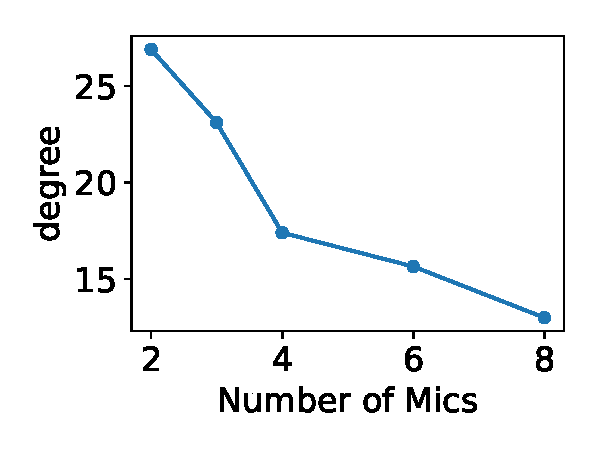
\includegraphics[width=0.75\linewidth]{chapters/cohear/evaluation/num_mics_orientation.pdf}
        \vspace{-1em}
        \caption{Orientation errors.}
        \label{fig:ori_mics}
    \end{subfigure}%
    \begin{subfigure}{0.48\linewidth}
        \centering
        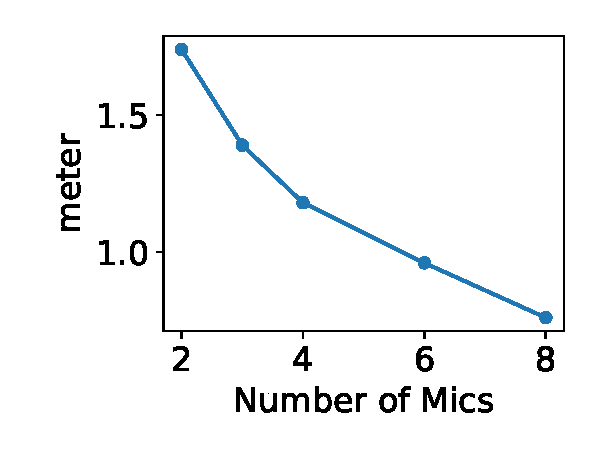
\includegraphics[width=0.75\linewidth]{chapters/cohear/evaluation/num_mics_position.pdf}
         \vspace{-1em}
        \caption{Position errors.}
        \label{fig:pos_mics}
    \end{subfigure}%
      \vspace{-1em}
    \caption{Geometric calibration with the number of microphones.}
    \label{fig:micro_mics}
    \vspace{-1em}
\end{figure}

\paragraph{Number of microphones}
The number of microphones has a significant impact on sound localization performance, which also affects the optimization of geometric calibration. To assess this, we conducted tests with different numbers of microphones. As shown in Fig. \ref{fig:micro_mics}, increasing the number of microphones leads to a decrease in estimation errors. Remarkably, even with only two microphones, the orientation estimation error is kept below 30 degrees.

\begin{figure}
    \centering
    \begin{subfigure}{0.48\linewidth}
        \centering
        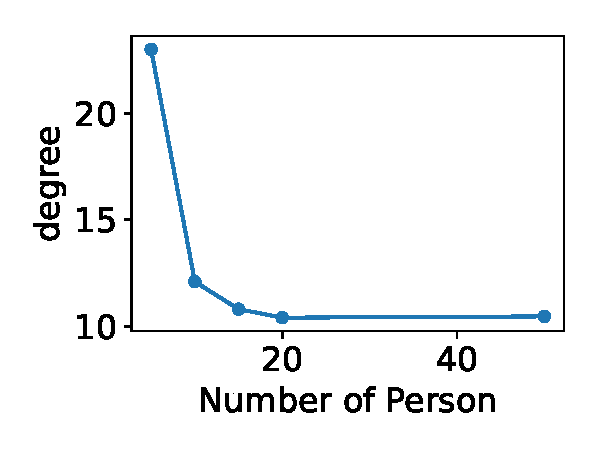
\includegraphics[width=0.75\linewidth]{chapters/cohear/evaluation/num_person_orientation.pdf}
         \vspace{-1em}
        \caption{Orientation errors.}
        \label{fig:ori_par}
    \end{subfigure}%
    \begin{subfigure}{0.48\linewidth}
        \centering
        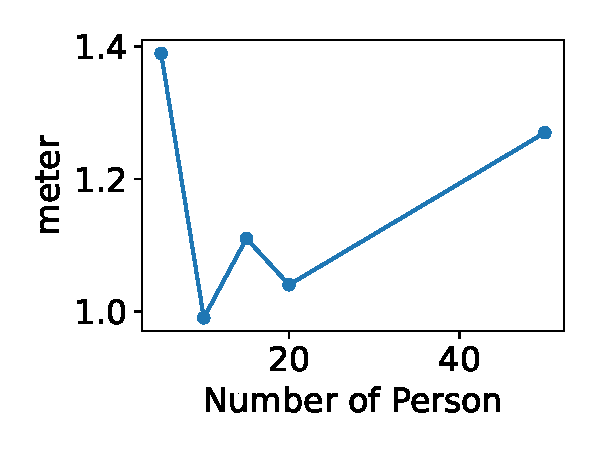
\includegraphics[width=0.75\linewidth]{chapters/cohear/evaluation/num_person_position.pdf}
         \vspace{-1em}
        \caption{Position errors.}
        \label{fig:pos_par}
    \end{subfigure}%
      \vspace{-1em}
    \caption{Geometric calibration with the number of participants.}
    \label{fig:micro_par}
     \vspace{-1em}
\end{figure}

\paragraph{Number of participants}
The number of participants appears to be closely related to the effectiveness of geometric calibration. However, as shown in Fig. \ref{fig:micro_par}, we observe a clear trend indicating that calibration error decreases with the number of participants, especially for the orientation error. Since the orientation accuracy is closely related to conversation accuracy, we conclude that CoHear can benefit from more participants.

\begin{figure}
    \centering
    \begin{subfigure}{0.48\linewidth}
        \centering
        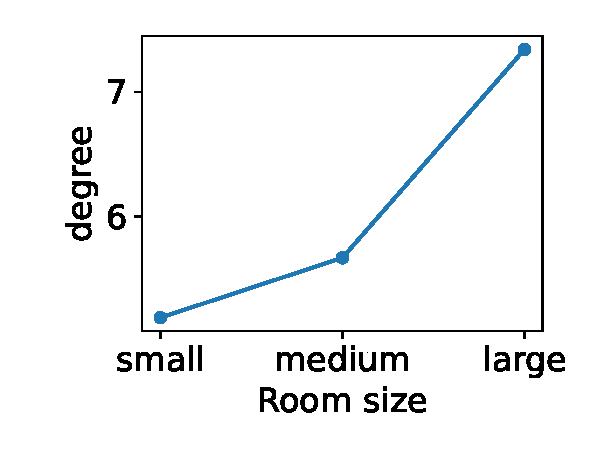
\includegraphics[width=0.75\linewidth]{chapters/cohear/evaluation/room_size_orientation.pdf}
         \vspace{-1em}
        \caption{Orientation errors.}
        \label{fig:ori_par}
    \end{subfigure}%
    \begin{subfigure}{0.48\linewidth}
        \centering
        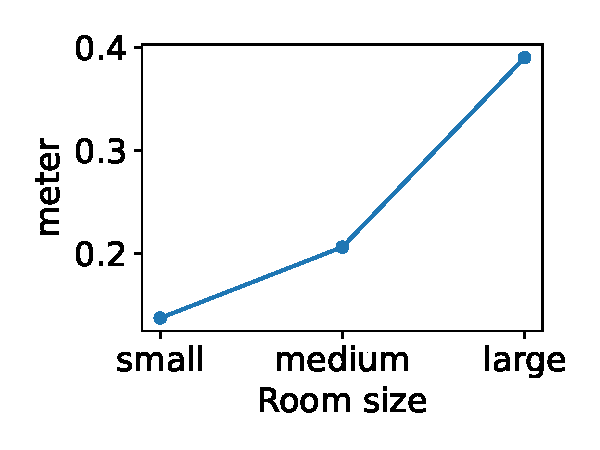
\includegraphics[width=0.75\linewidth]{chapters/cohear/evaluation/room_size_position.pdf}
         \vspace{-1em}
        \caption{Position errors.}
        \label{fig:pos_par}
    \end{subfigure}%
      \vspace{-1em}
    \caption{Geometric calibration with the size of rooms.}
    \label{fig:micro_size}
     \vspace{-1em}
\end{figure}

\paragraph{Size of room}
The size of the room affects the distance between users (while keeping the number of users constant), which in turn impacts the performance of the geometric calibration. To investigate this, we tested three room sizes: small (5x5 to 10x10 meters), medium (10x10 to 15x15 meters), and large (15x15 to 20x20 meters). As shown in Fig. \ref{fig:micro_size}, the results show a clear trend of increasing error with room size. This matches our expectation, as users positioned closer together lead to better calibration performance.

\begin{figure}
    \centering
    \begin{subfigure}{0.48\linewidth}
        \centering
        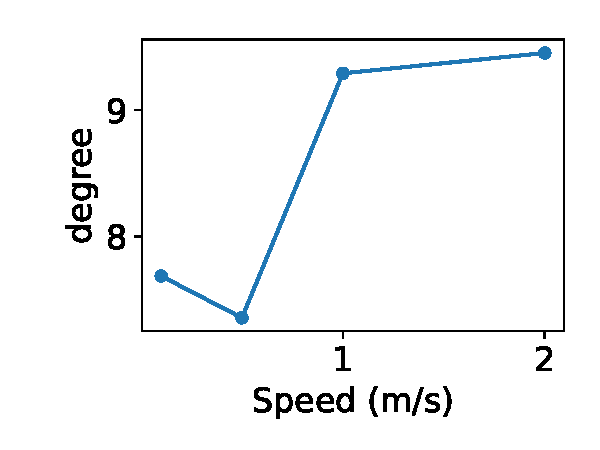
\includegraphics[width=0.75\linewidth]{chapters/cohear/evaluation/speed_orientation.pdf}
         \vspace{-1em}
        \caption{Orientation errors.}
        \label{fig:ori_speed}
    \end{subfigure}%
    \begin{subfigure}{0.48\linewidth}
        \centering
        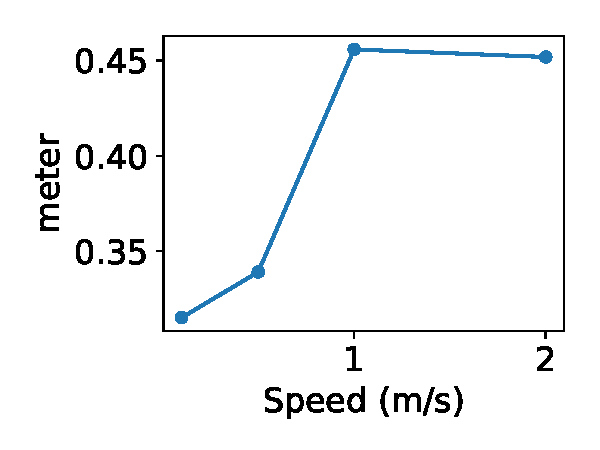
\includegraphics[width=0.75\linewidth]{chapters/cohear/evaluation/speed_position.pdf}
         \vspace{-1em}
        \caption{Position error.}
        \label{fig:pos_speed}
    \end{subfigure}%
     \vspace{-1em}
    \caption{Geometric calibration with movement speed.}
    \label{fig:micro_speed}
    \vspace{-1em}
\end{figure}


\paragraph{Movement speed}
The movement of participants can affect the geometric calibration by altering the observations. We find that moving speed is a key factor that distinguishes CoHear from static WASN, which can be considered as having a speed of 0. In Fig. \ref{fig:micro_speed}, we present the localization errors at various speed levels. Our findings indicate that speed may not have a significant impact on geometric calibration, demonstrating that our system is robust across different speeds.


\begin{figure}[htbp]
    \centering
    \begin{minipage}{0.45\linewidth}
        \centering
        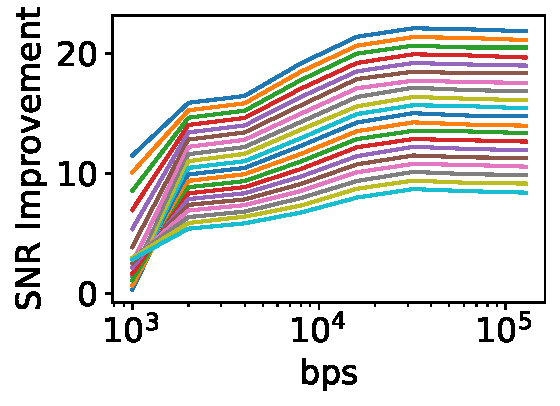
\includegraphics[width=0.7\linewidth]{chapters/cohear/figs/opus_benchmark.pdf}
        \vspace{-1em}
        \caption{Conversation enhancement under different bandwidth, where each line refers to different levels of input SNR.}
        \label{fig:measurement1}
    \end{minipage}
    \hfill
    \begin{minipage}{0.45\linewidth}
        \centering
        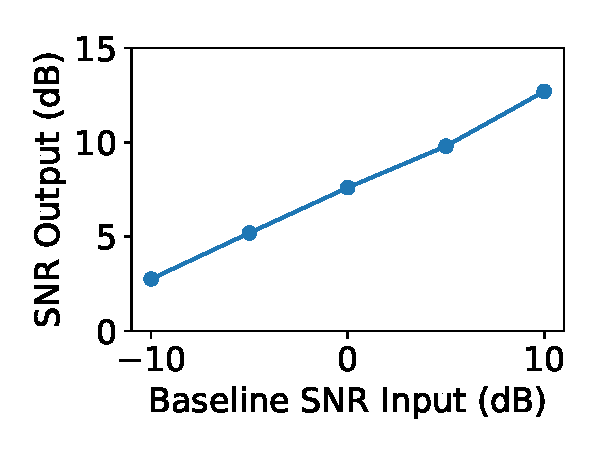
\includegraphics[width=0.7\linewidth]{chapters/cohear/figs/baseline.pdf}
        \vspace{-1em}
        \caption{Conversation enhancement with time-invariant feature only.}
        \label{fig:baseline_measurement}
    \end{minipage}
    \vspace{-1em}
\end{figure}

\paragraph{Bandwidth}
We evaluate the correlation between performance and compression ratios at different interference levels in Fig. \ref{fig:measurement1}. For each line that refers to one input SNR, we observe that the relationship between bandwidth and performance does not follow a straightforward linear pattern.
To further reduce bandwidth usage, we can rely solely on the speaker embedding when performance is adequate, and we conducted an additional evaluation in Fig. \ref{fig:baseline_measurement}. If the output at 10 dB is considered satisfactory, our observations indicate that enabling the speaker embedding when the input SNR exceeds 5 dB is sufficient, indicating the adaptability of CoHear with constrained network.


\begin{figure}
    \centering
    % First row
    \begin{subfigure}{0.48\linewidth}
        \centering
        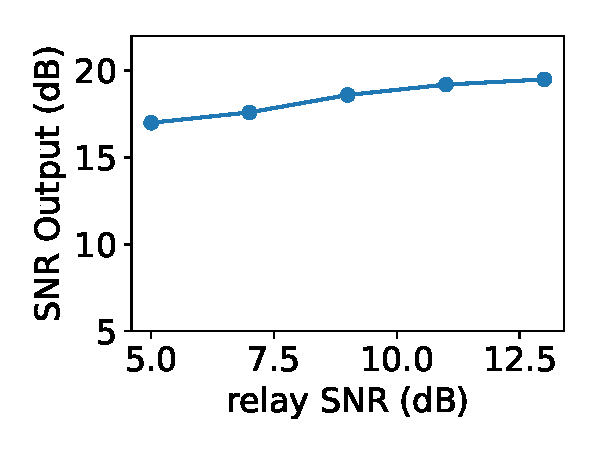
\includegraphics[width=0.75\linewidth]{chapters/cohear/evaluation/relay_snr.pdf}
         \vspace{-1em}
         \caption{}
        \label{fig:relay_snr}
    \end{subfigure}%
    \begin{subfigure}{0.48\linewidth}
        \centering
        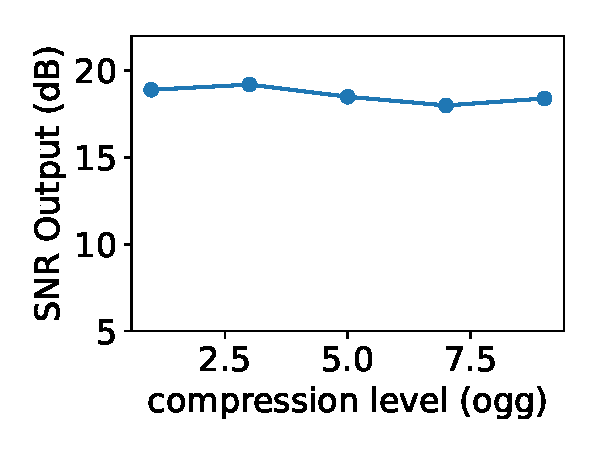
\includegraphics[width=0.75\linewidth]{chapters/cohear/evaluation/compression_quality.pdf}
         \vspace{-1em}
          \caption{}
        \label{fig:relay_compress}
    \end{subfigure}

    % Second row
    \begin{subfigure}{0.48\linewidth}
        \centering
        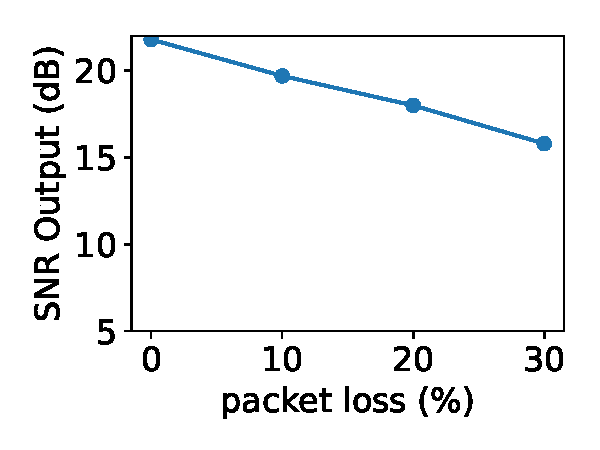
\includegraphics[width=0.75\linewidth]{chapters/cohear/evaluation/packet_loss.pdf}
         \vspace{-1em}
         \caption{}
        \label{fig:relay_packet}
    \end{subfigure}%
    \begin{subfigure}{0.48\linewidth}
        \centering
        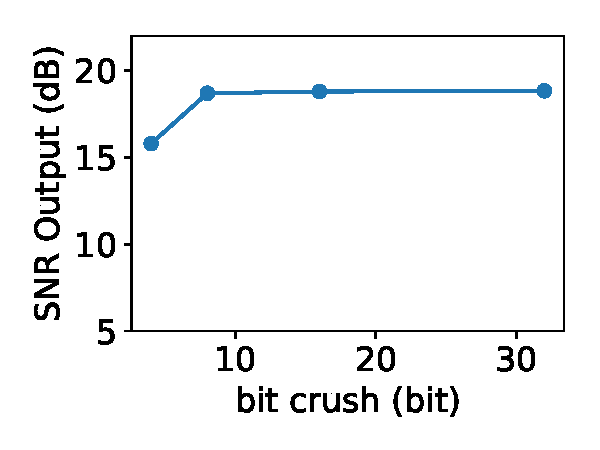
\includegraphics[width=0.75\linewidth]{chapters/cohear/evaluation/bit_crush.pdf}
         \vspace{-1em}
         \caption{}
        \label{fig:relay_bit}
    \end{subfigure}
      \vspace{-1em}
    \caption{Micro-benchmark of conversation extraction under various perturbations on the relay audio.}
    \label{fig:relay_audio_quality}
        \vspace{-1em}
\end{figure}

\paragraph{Relay audio quality}
In the design of CoHear, we utilize relay audio as a condition instead of speaker embedding. This choice emphasizes that the quality of the relay audio is critical for the system's performance, which we assess across four aspects, as illustrated in Fig. \ref{fig:relay_audio_quality}.
As shown in Fig. \ref{fig:relay_snr}, there is a positive correlation between the SNR of the relay audio and overall performance. This finding indicates that CoHear relies on effective self-voice isolation algorithms, such as VibVoice or ClearBuds \cite{chatterjee2022clearbuds, he2023towards}. Regarding compression quality (Fig. \ref{fig:relay_compress}), we observe that it has only a slight impact on performance, demonstrating that CoHear is resilient to compression effects.
The remaining two factors are related to wireless transmission. We note that packet loss negatively affects performance (Fig. \ref{fig:relay_packet}), whereas the bit-crush effect stabilizes at 8 bits (Fig. \ref{fig:relay_bit}). This suggests that we can standardize the transmitted bit width to eight bits without compromising performance.

\paragraph{Number of participants}
Considering that a conversation can involve multiple participants, we also evaluate the performance degradation as the number of speakers increases, as shown in Fig. \ref{fig:num_conditions}. We observe that performance declines slightly with more speakers, which aligns with our intuition.


\begin{figure}
    \centering
    \begin{minipage}{0.48\linewidth}
        \centering
        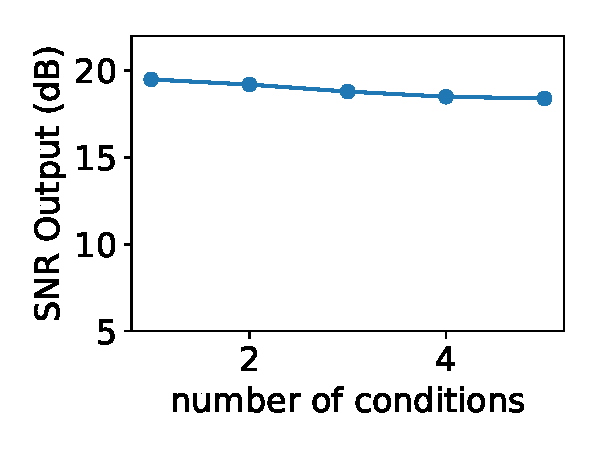
\includegraphics[width=0.75\linewidth]{chapters/cohear/evaluation/num_conditions.pdf}
         \vspace{-1em}
    \caption{Conversation extraction with the number of participants.}
    \label{fig:num_conditions}
    \end{minipage}%
    \hfill
    \begin{minipage}{0.48\linewidth}
        \centering
        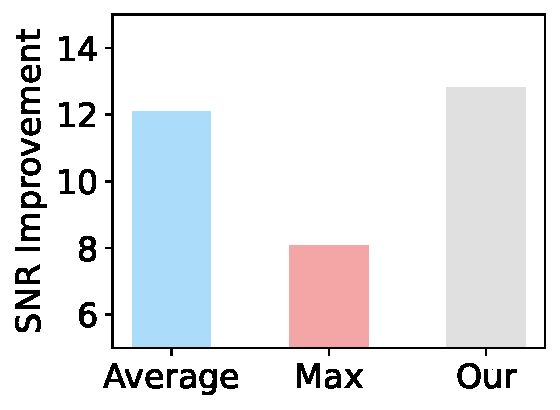
\includegraphics[width=0.75\linewidth]{chapters/cohear/figs/controller.pdf}
         \vspace{-1em}
        \caption{Conversation extraction with bandwidth controller.}
        \label{fig:controller}
    \end{minipage}
    \vspace{-1em}
\end{figure}

\subsection{System Overhead}

\begin{figure}
    \centering
    \begin{subfigure}{0.48\linewidth}
        \centering
        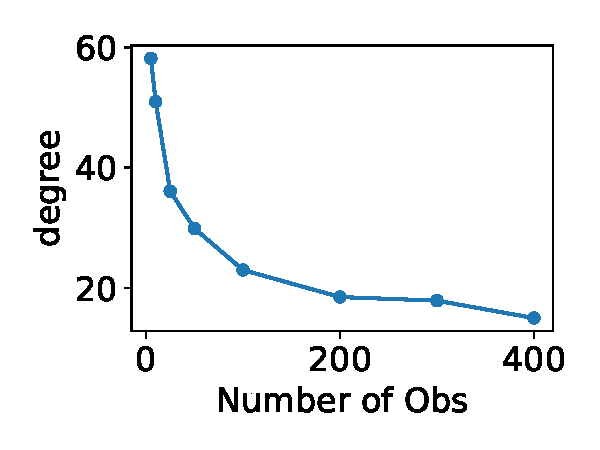
\includegraphics[width=0.75\linewidth]{chapters/cohear/evaluation/num_obs_orientation.pdf}
         \vspace{-1em}
        \caption{Orientation errors.}
        \label{fig:num_obs_orientation}
    \end{subfigure}%
    \begin{subfigure}{0.48\linewidth}
        \centering
        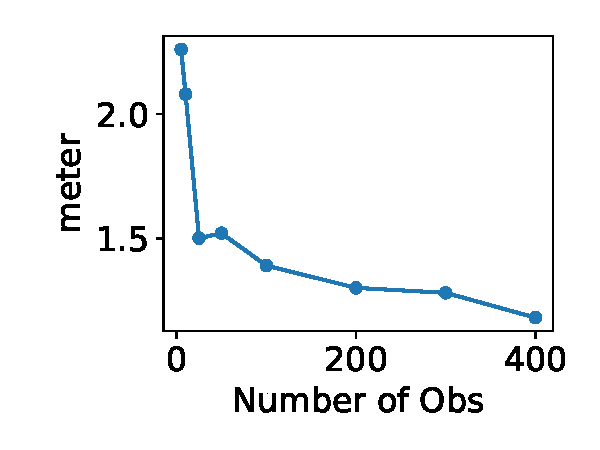
\includegraphics[width=0.75\linewidth]{chapters/cohear/evaluation/num_obs_position.pdf}
         \vspace{-1em}
        \caption{Position errors.}
        \label{fig:num_obs_position}
    \end{subfigure}
     \vspace{-1em}
    \caption{Geometric calibration with increasing number of observations.}
    \label{fig:num_obs}
    \vspace{-1em}
\end{figure}

\paragraph{Bandwidth controller}
We assess the performance of our experience-based controller as shown in Fig. \ref{fig:controller}. In this comparison, we evaluate it against two naive baselines: one where each stream receives equal bandwidth, and another where the first stream receives the maximum bandwidth while the second stream receives the remaining bandwidth, so on and so forth. During our experiments, we utilized a random number of nodes, random input SNR, and random available bandwidth. The average SNR is displayed in the figure. Our findings indicate that the proposed controller can achieve an improvement of approximately 1 dB without requiring additional bandwidth.

\paragraph{Cold start time}
CoHear depends on a sufficient number of observations or utterances to accurately calibrate the locations of participants. This means that there is a "cold start" period during which the system needs time to achieve optimal performance, as indicated by the conversation accuracy discussed in the previous section.
In Fig. \ref{fig:num_obs}, we present both orientation errors and position errors. Our findings show that CoHear requires only a few observations (specifically, around 50) to achieve good results, particularly in orientation estimation.


\paragraph{Runtime latency}
CoHear is designed to provide a real-time experience for users, meaning that it is good to have less latency. Since we can process data at the frame level, it is crucial to keep the frame length under 50 ms and ensure that the real-time factor is greater than 1.
We tested the latency on both a smartphone (Pixel 7) and a desktop computer, using either a CPU (i7-11700k) or a GPU (RTX 3090). The results show that the real-time factor (the time to process one frame divided by the duration of the frame) is 2 on the smartphone, 10 on the desktop CPU, and 1250 on the desktop GPU. Compared to baselines such as \cite{veluri2024look}, our system exhibits similar overhead since the majority of the neural network architecture is the same, with only additional computation required for the encoder.

It is also important to note that we do not include the latency of geometric calibration in our real-time inference measurements, as this process can be performed on a server in parallel and takes only 0.2 seconds for 100 observations.





